\section{Proposed Method}
\label{proposed_method}
\subsection{Apriori-window}
Dense patterns denote itemsets with high local occurrence frequencies. 
It is impractical to determine whether a pattern is dense for all combinations of items that appear in transaction data due to combinatorial explosion. 
Therefore, it is necessary to limit the target of pattern evaluation to a set of itemsets whose occurrences are locally concentrated. 
The method exploits Apriori’s anti-monotonicity\cite{agrawal1994fast}: if an itemset fails to meet the minimum interval support ($minSup$) and minimum interval length ($minL$) criteria, every superset thereof is automatically invalid. By leveraging this property, the conventional Apriori framework is adapted for dense pattern extraction, resulting in the exact algorithm \emph{Apriori-window} that exhaustively enumerates these patterns.
We prove below that anti-monotonicity holds in dense patterns.

\begin{proof}[Proof of the Anti-monotonicity in Dense Patterns]
Let \( D = [d_1, \dots, d_N] \) be a transaction dataset with each transaction represented as \( d_i = (ts_i, X_{ts_i}) \), and let the ordered list of timestamps be \( T = [ts_1, \dots, ts_N] \). For any interval \( I = [ts_i, ts_j] \) with length $n(D_I) = j - i + 1 \ge \textit{minL}$,
denote the corresponding sequence of itemsets by
$D_I = [X_{ts_i}, \dots, X_{ts_j}]$.

Assume that an itemset \( P \) is not a dense pattern; that is, for every interval \( I \) with \( n(D_I) \ge \textit{minL} \), we have
$Sup_I(P) < \textit{minSup}$.
Consider any extension \( P' \) such that \( P \subset P' \). For any interval \( I \), define
$T(P'; I) = \{ X \in D_I \mid P' \subseteq X \}$
as the set of transactions in \( I \) containing \( P' \), and similarly define
$T(P; I) = \{ X \in D_I \mid P \subseteq X \}$.
Since every transaction that contains \( P' \) also contains \( P \), it follows that
$T(P'; I) \subseteq T(P; I)$.
Thus, we have
$n\bigl(T(P'; I)\bigr) \le n\bigl(T(P; I)\bigr)$,
which implies
\[
Sup_I(P') = \frac{n\bigl(T(P'; I)\bigr)}{n(D_I)} \le \frac{n\bigl(T(P; I)\bigr)}{n(D_I)} = Sup_I(P).
\]
Consequently, for every interval \( I \) with \( n(D_I) \ge \textit{minL} \),
\[
Sup_I(P') \le Sup_I(P) < \textit{minSup}.
\]
Furthermore, since the occurrence positions of \( P' \) form a subset of those of \( P \), if no contiguous interval of length at least \(\textit{minL}\) exists for \( P \) (i.e., no \( I \) with \( n(D_I) \ge \textit{minL} \) satisfies \( Sup_I(P) \ge \textit{minSup} \)), then none exists for \( P' \) either.

Therefore, any extension \( P' \) of an itemset \( P \) that is not a dense pattern will necessarily fail to meet the conditions
\[
Sup_I(P') \ge \textit{minSup} \quad \text{and} \quad n(D_I) \ge \textit{minL},
\]
thereby establishing the anti-monotonicity of dense patterns.
\end{proof}



\begin{algorithm}[t]
    \makeatletter
    \renewcommand{\algorithmicrequire}{\textbf{Input:}}
    \renewcommand{\algorithmicensure}{\textbf{Output:}}
    \makeatother
    \begin{algorithmic}[1]
    \caption{Main Algorithm of Apriori-window}
    \label{alg:apriori-window}
        \Require Dataset $D$, minimum interval support $minSup$, minimum interval length $minL$
        \Ensure Set of dense patterns $L$ and their occurrence intervals
        \State $L \gets \{\}$
        % \Comment{Initialize the set of dense patterns}
        \State Evaluate each single item by sliding window mechanism.
        \State Add the length-$1$ dense pattern and its dense intervals to $L(1)$.
        \For{$k \gets 2$ \textbf{to} $L(k-1) \neq \emptyset$}
            \State $L(k) \gets \{\}$
            \State $C_k \gets \{\}$ 
            % \Comment{Initialize the candidate set for itemsets of length $k$}
            \State Generate all candidate itemsets of length $k$ from $L(k-1)$.
            \State Add the candidate itemsets to $C_k$.
            \For{each candidate in $C_k$}
                \State Evaluate the candidate by the sliding window mechanism.
                \State Add the length-$k$ dense patterns and its dense intervals to $L(k)$.
            \EndFor
        \EndFor
        \State \Return $\bigcup_k L(k)$
    \end{algorithmic}
\end{algorithm}


Algorithm~\ref{alg:apriori-window} presents the core procedure of the Apriori-window algorithm. In the initial phase, the algorithm scans the occurrence positions of each item using a sliding window mechanism. This mechanism utilizes a fixed-width window that moves sequentially over the transaction data, precisely capturing local frequency variations. Within each window, it evaluates the occurrence frequency of items and merges overlapping dense intervals, thereby extracting dense single-item patterns.A detailed description of the sliding window mechanism is provided in Algorithm~\ref{alg/sliding_window_mechanism}.

Subsequently, candidate patterns of length two or more are generated by leveraging the Apriori property based on these dense single-item patterns. Each candidate is then assessed by the same sliding window mechanism, ensuring that local density is accurately measured while redundant evaluations are minimized.

Moreover, the module incorporates a stride adjustment technique (lines 17 to 19 in Algorithm \ref{alg/sliding_window_mechanism}) to enhance computational efficiency. When the support within a window exceeds the threshold, the surplus is used to determine an increased stride, thereby allowing the algorithm to skip redundant windows. 

\begin{algorithm}[t] 
    \caption{Sliding Window Mechanism} 
    \label{alg/sliding_window_mechanism}

    \makeatletter 
    \renewcommand{\algorithmicrequire}{\textbf{Input:}} 
    \renewcommand{\algorithmicensure}{\textbf{Output:}} 
    \makeatother
    
    \begin{algorithmic}[1] 
        \Require Occurrence positions for all items $positions$, itemset $X$, minimum interval support $minSup$, minimum interval length $minL$ 
        \Ensure List of dense intervals $C$ for the itemset $X$
    
        \State $W \gets minL$ 
        % \Comment{Set the width of the sliding window} 
        \State $positions(X) \gets$ List of occurrence positions of itemset $X$ (sorted in ascending order)
        \State $C \gets$ Empty list 
        % \Comment{Initialize the list of dense intervals}
        
        \For{$i \gets 0$ to $|positions(X)| - W -1$} 
            \State $window_{start} \gets positions(X)[i]$ 
            \State $window_{end} \gets window_{start} + W$ 
            \State $count \gets 0$ 
            \For{$j \gets i$ to $|positions(X)| - 1$} 
                \If{$positions(X)[j] < window_{end}$} 
                    \State $count \gets count + 1$ 
                \Else 
                    \State \textbf{break} 
                \EndIf 
            \EndFor 
            \If{$\dfrac{count}{W} \geq minSup$} 
                \State Add dense interval $[window_{start}, window_{end}]$ to $C$
                \State $surplus \gets support - minSup$ 
                % \Comment{Calculate the surplus of the interval support}
                \State $skip \gets \text{floor}(W \times surplus)$ 
                % \Comment{Obtain the integer part of the surplus using the floor function}
                \State $i \gets i + \max(1, skip) - 1$ 
                % \Comment{Determine the starting position of the next window}
            \EndIf
        \EndFor
        
        \State $C \gets$ Merge overlapping or adjacent dense intervals 
        \State \Return $(X,~C)$
        
    \end{algorithmic} 
\end{algorithm}


\subsection{Plant Model}
% We propose \emph{Plant Model} as a novel approach for extracting densely occurring patterns. 
% We implement a \emph{candidate extraction module} inspired by swarm intelligence to efficiently extract pairs of dense itemset candidates and their dense interval candidates.
% Subsequently, we apply a \emph{pattern evaluation module} to rigorously detect the dense intervals for each candidate, thereby identifying the dense patterns.
% The candidate extraction module and the pattern evaluation module are iteratively executed to output all extracted dense patterns and their dense intervals at the end of the process.


We propose the \emph{Plant Model} as a novel approach for extracting densely occurring patterns. It consists of two main components: a \emph{candidate extraction module}, inspired by swarm intelligence, and a \emph{pattern evaluation module} for rigorously detecting dense intervals. Fig.~\ref{fig:entire-flow} shows the flow chart of the proposed Plant Model.
The candidate extraction module extracts pairs of dense itemset candidates and their corresponding dense interval candidates. Subsequently, the pattern evaluation module applies rigorous detection to each candidate, thereby identifying the dense patterns. These modules are iteratively executed executed to output all extracted dense patterns and their dense intervals at the end of the process.

\begin{figure}[t]
    \centering
    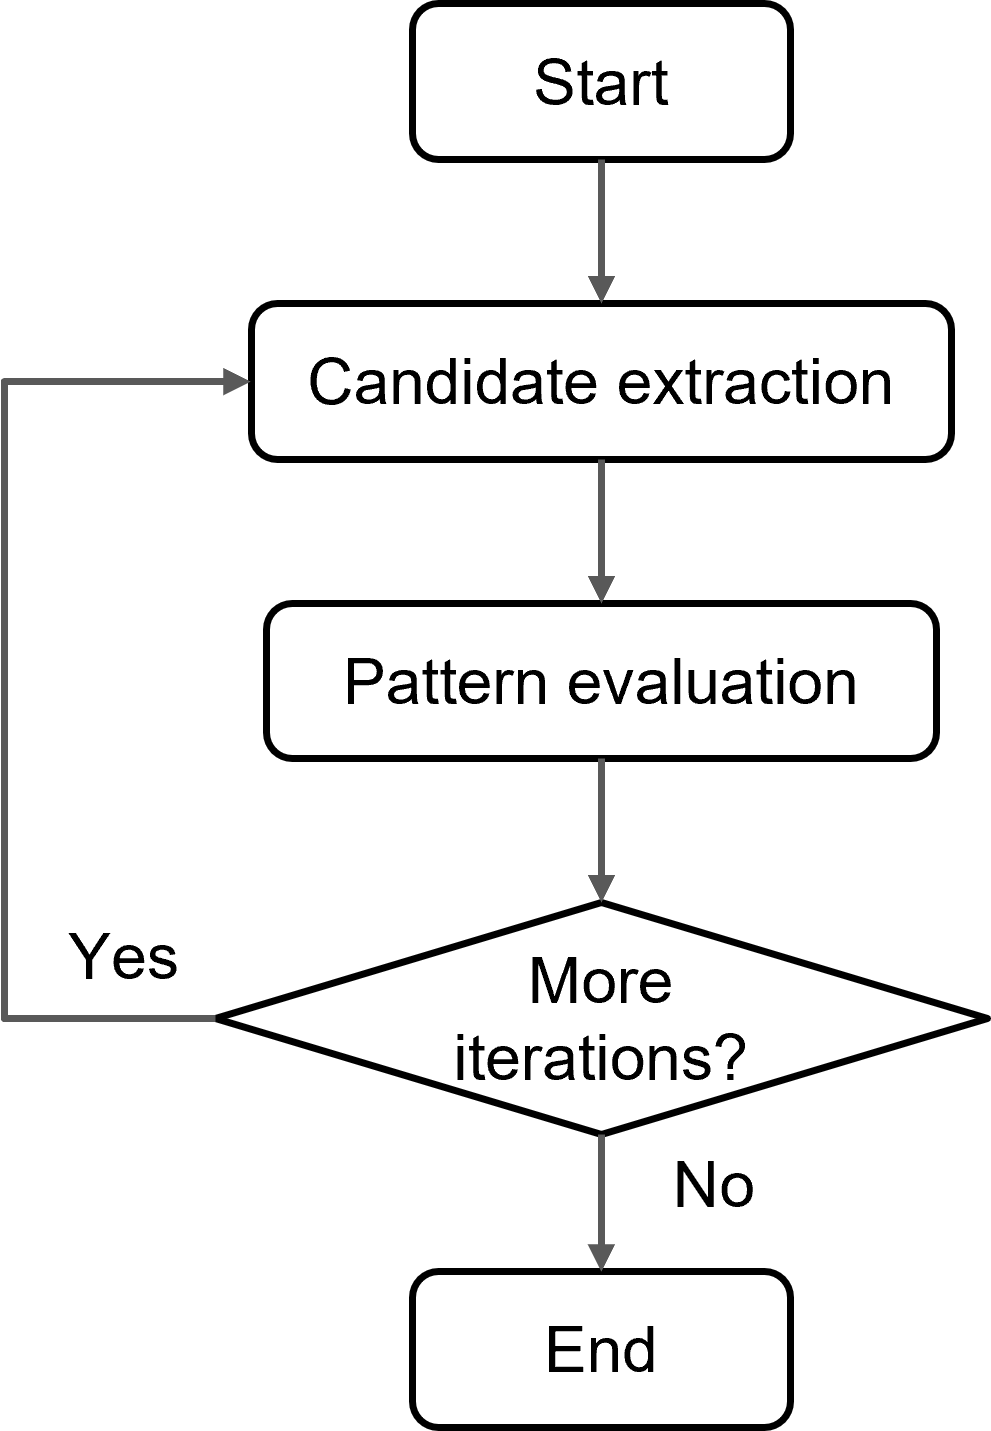
\includegraphics[width=0.5\linewidth]{fig/entire_flow.png}
    \caption{Flow chart of proposed Plant Model. The candidate extraction module and the pattern evaluation module are executed in sequence and repeated until the early termination condition is satisfied or the maximum number of iterations is reached.}
    \label{fig:entire-flow}
\end{figure}

\subsubsection{Candidate Extraction Module}

\begin{figure}
    \centering
    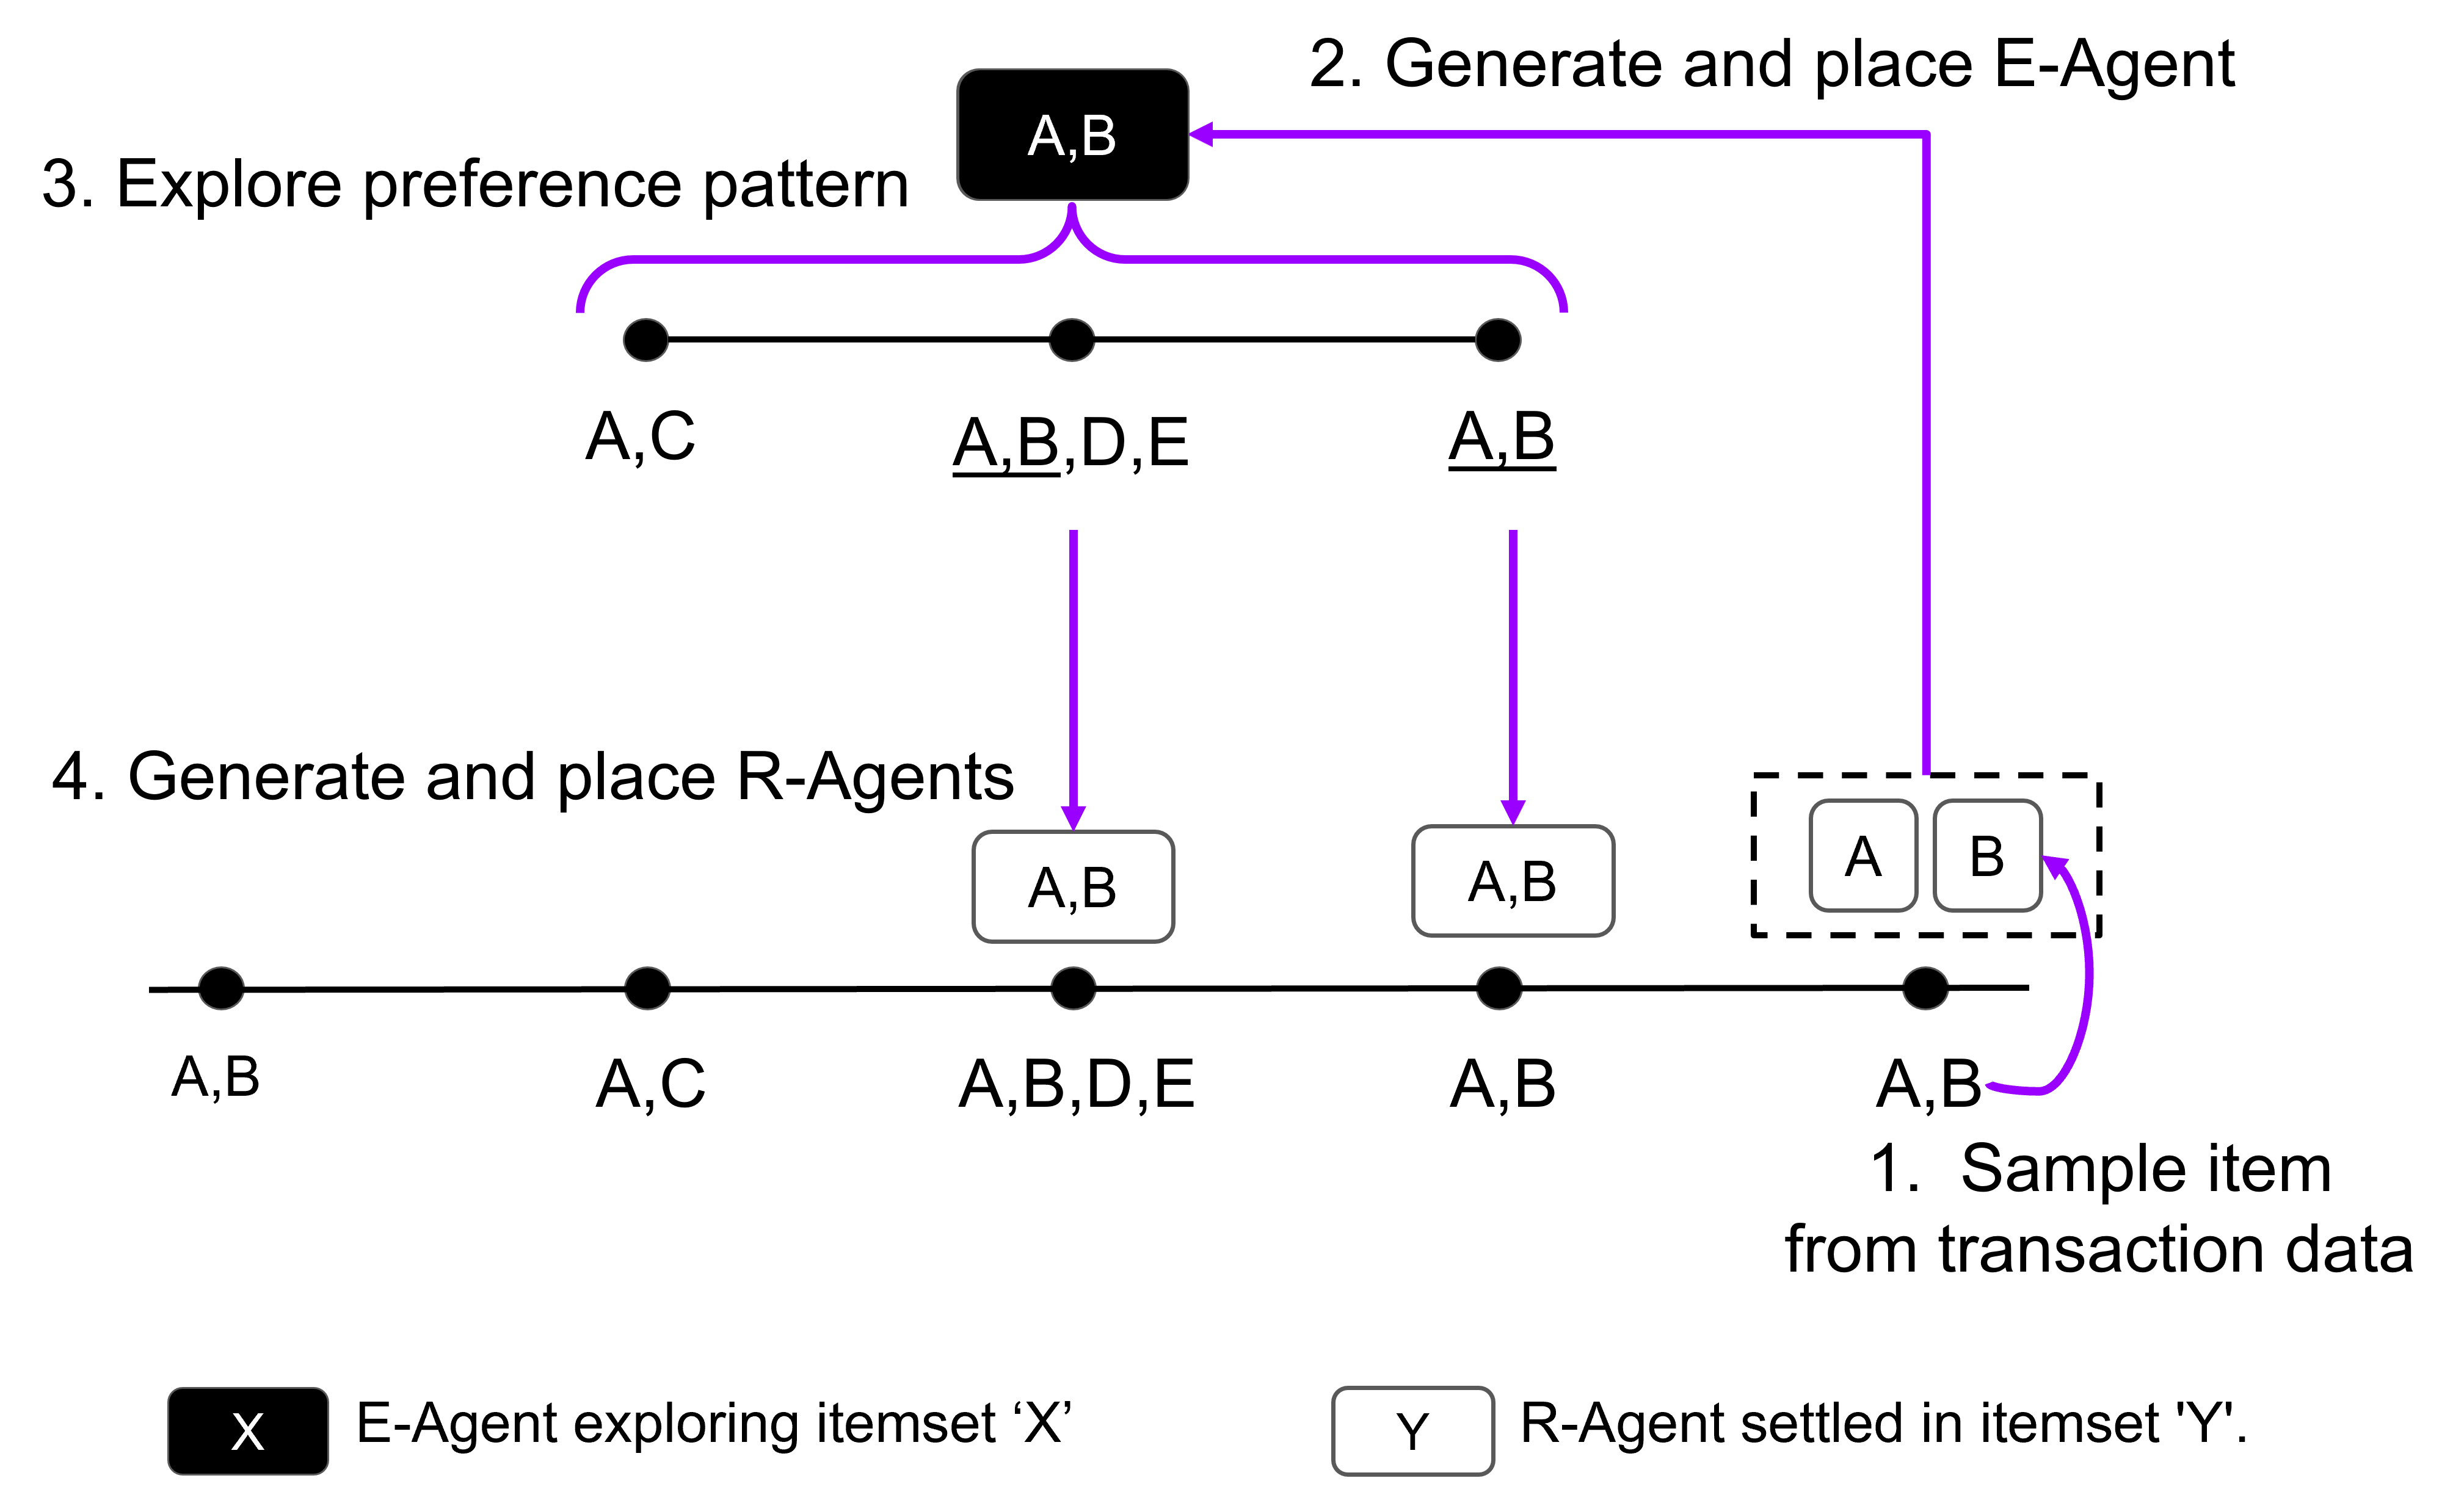
\includegraphics[width=1\linewidth]{fig/candidate-extraction-module.png}
    \caption{Behavior of the two types agent in the candidate extraction module. The strings written within each agent represent preference patterns.  After executing the steps 1 through 4, the distribution of R-Agents is aggregated and candidate patterns and their dense intervals are selected. This cycle is resumed after pattern identification in the pattern evaluation module.}
    \label{fig:candidate-extract}
\end{figure}

The objective of the candidate extraction module is to identify itemsets and corresponding concentrated intervals that are likely to be judged as dense patterns. To find these candidate patterns, the module takes a swarm intelligence-based bottom-up search approach. This approach is inspired by the behavior of plants that expand their habitat through hybridization. Specifically, the module finds itemsets that appear at dense intervals from other itemsets within the transaction to which the items sampled from transaction data belongs or nearby.

The candidate extraction module consists of two types of agents: \emph{R-Agents} (resident-agent) and \emph{E-Agents} (explore-agent). The R-Agent functions as a marker by indicating the transaction in which each item appears. The E-Agent, on the other hand, is responsible for searching for occurrences of the target item set within the transactions adjacent to the assigned timestamp.


In order to search for candidate patterns, the process is decomposed into several sequential steps, as shown in Fig.~\ref{fig:candidate-extract}. Initially, unit R-Agents are deployed using items randomly extracted from the dataset(step 1 in Fig.~\ref{fig:candidate-extract}). Each of these agents retains its respective item as a preference pattern, thereby serving as the starting point for subsequent exploration. 
Next, each R-Agent consults its own preference pattern along with that of neighboring R-Agents to determine the itemset to be explored in the next time step. The determined itemset is then set as the preference pattern for the E-Agents in the subsequent phase. This determination process adopts one of two modes: a replication mode, which preserves the current preference pattern unchanged, or a synthesis mode, which outputs the union of the preference patterns.E-Agents generated by the above process are probabilistically placed near the position of the parent R-Agent (step 2 in Fig.~\ref{fig:candidate-extract}).
Once deployed, these E-Agents actively search within a predetermined region for the occurrence of itemsets that match their preference patterns(step 3 in Fig.~\ref{fig:candidate-extract}). When an E-Agent detects a transaction containing the target itemset, it places a new R-Agent at that transaction(step 4 in Fig.~\ref{fig:candidate-extract}).

Finally, the number of R-Agents associated with each itemset is aggregated, and if this count exceeds a  minimum occurrence threshold($= minSup \times minL$), the corresponding itemset is selected as a candidate pattern. The spatial distribution of all R-Agents associated with the selected itemset is then defined as the candidate dense interval for that pattern.

After the pattern evaluation phase, the candidate extraction process is iteratively repeated. This cyclical generation ultimately results in the extraction of densely occurring patterns with localized concentrations, along with their corresponding dense intervals.
Itemsets that are determined to be dense patterns are suppressed from being selected as preferred patterns in the candidate extraction module. In this paper, we distinguish two variants of the Plant Model by their suppression strategy:
\begin{itemize}
  \item \emph{Plant Model (Global Suppression)}: Once an itemset is judged to be dense, its occurrences are suppressed across the entire transaction dataset.
  \item \emph{Plant Model (Interval‑Restricted Suppression)}: Suppression is applied only within the detected dense interval of the pattern.
\end{itemize}


\begin{algorithm}[t] 

    \makeatletter 
    \renewcommand{\algorithmicrequire}{\textbf{Input:}} 
    \renewcommand{\algorithmicensure}{\textbf{Output:}} 
    \makeatother
    
    \begin{algorithmic}[1]
    \caption{Candidate Extraction Module} 
    \label{alg:candidate-extraction-module}
        \Require Transaction data $D$, maximum pattern length $plength_{max}$, unit R-Agent number $pop_{btm}$, R-Agent sampling number $N_{sampling}$, exploration range radius $r$, scan waiting cycle count $w_{scan}$, replication probability $prob_{copy}$, tentative pattern candidate set $C_{tentative}$, E-Agents list $Agents_{explore}$, dense pattern set $L$, minimum occurrence threshold $minfreq$
        \Ensure List of pairs (pattern candidate, candidate region) $P$, tentative pattern candidate set $C_{tentative}$, E-Agents list $Agents_{explore}$
        
        \State $P \gets \{\}$ 
        % \Comment{Initialize the set of pattern candidates and their regions}

        \State $Agents_{resident} \gets \{\}$
        \State Generate and deploy unit R-Agents.
        \State Add the generated unit R-Agents to $Agents_{resident}$.
        
        \For{$Agent_{explore}$ \textbf{in} $Agents_{explore}$}
            \State Generate and deploy R-Agents.
            \State Add the generated R-Agents to $Agents_{resident}$.
        \EndFor
        
        \State Delete all E-Agents.
        \State Delete all R-Agents that have attempted the discovered dense patterns.
        \State Add itemsets with R-Agent count $\geq minfreq$ to $C_{tentative}$ 
        % \Comment{Record tentative pattern candidates}
        
        \For{$candidate$ \textbf{in} $C_{tentative}$}
            \If{the waiting cycle count of $candidate$ $\geq w_{scan}$}
                \State Add ($candidate$, list of occurrence positions) to $P$ 
                % \Comment{Record the pair of pattern candidate and candidate region}
            \Else
                \State the waiting cycle count of $candidate$ ++.
            \EndIf
        \EndFor
        
        \State Sample R-Agents.
        \For{$Agent_{resident}$ \textbf{in} $Agents_{resident(sampled)}$}
            \State Generate a new pattern $F_{new}$.
            \State Generate and deploy E-Agents.
            \State Add the generated E-Agents to $Agents_{explore}$.
        \EndFor
        
        \State Delete all R-Agents.
        
        \State \Return $P$, $C_{tentative}$, $Agents_{explore}$
    \end{algorithmic}
\end{algorithm}


\subsubsection{Pattern Evaluation Module}
% \input{alg/pattern_evaluation_module}

The pattern evaluation module is introduced to accurately extract truly dense patterns from the R-Agent location data produced by the candidate extraction module.
The input to the pattern evaluation module, denoted as \(positions\), is a sorted list of the R-Agents’ fixed positions corresponding to the transactions in which each candidate pattern occurs. The module applies a sliding window mechanism as well as Apriori-window over \(positions\) to detect dense intervals. 



\subsubsection{Termination Conditions}
In addition to termination by the predefined maximum iterations, the Plant Model introduces early termination. If no new dense patterns are extracted after the start of the run or after the last dense pattern is extracted for one-fifth of the maximum number of cycles, the model terminates early without waiting for the maximum iterations to elapse.

\subsubsection{Hyperparameters}
The attributes of the two types of agents and the number of agents produced are based on the hyperparameters listed in Table \ref{tab:plant_params}. Maximum Iterations defines the maximum number of cycles to be completed. No. of Unit R-Agents specifies the number of unit R-Agents generated in each cycle. R-Agent Sampling Count specifies the number of R-Agents that generate E-Agents. Exploration Range Radius specifies the range to be searched by each E-Agent. Scan Wait Cycle Count specifies the number of waiting cycles from the time a candidate is registered as a pattern candidate to the time it is evaluated. Replication Probability specifies the probability that a R-Agent chooses the replication mode when generating preference patterns.

\begin{table}[t]
    \centering
    \caption{Hyperparameters of Plant Model}
    \begin{tabular}{|c|c|}
        \hline
        \textbf{Hyperparameter} & \textbf{Description} \\
        \hline
        Maximum Iterations & 
        \begin{tabular}{@{}l@{}}
            The maximum number of cycles \\
            until termination
        \end{tabular} \\\hline
        No. of Unit R-Agents & 
        \begin{tabular}{@{}l@{}}
            The number of unit R-Agents \\
            generated in each epoch
        \end{tabular} \\\hline
        R-Agent Sampling Count &
        \begin{tabular}{@{}l@{}}
            The number of R-Agents available \\
            for generating exploratory agents
        \end{tabular} \\\hline
        Exploration Range Radius & 
        \begin{tabular}{@{}l@{}}
            The range within which \\
            the E-Agents search
        \end{tabular} \\\hline
        Scan Wait Cycle Count & 
        \begin{tabular}{@{}l@{}}
        The number of cycles to wait \\for pattern candidate registration
        \end{tabular} \\\hline
        Replication Probability &
        \begin{tabular}{@{}l@{}}
            The probability of selecting\\ the replication mode\\
            during preference pattern generation
        \end{tabular} \\
        \hline
    \end{tabular}
    \label{tab:plant_params}
\end{table}
